\documentclass{beamer}

%%{ header

\mode<presentation> {

  %%{ themes

  % \usetheme{default}
  % \usetheme{annarbor}
  % \usetheme{antibes}
  % \usetheme{bergen}
  % \usetheme{berkeley}
  % \usetheme{berlin}
  % \usetheme{boadilla}
  % \usetheme{cambridgeus}
  % \usetheme{copenhagen}
  % \usetheme{darmstadt}
  % \usetheme{dresden}
  % \usetheme{frankfurt}
  % \usetheme{goettingen}
  % \usetheme{hannover}
  % \usetheme{ilmenau}
  % \usetheme{juanlespins}
  % \usetheme{luebeck}
  % \usetheme{madrid}
  % \usetheme{malmoe}
  % \usetheme{marburg}
  % \usetheme{montpellier}
  % \usetheme{paloalto}
  % \usetheme{pittsburgh}
  % \usetheme{rochester}
  % \usetheme{singapore}
  % \usetheme{szeged}
  % \usetheme{warsaw}
  % \usetheme{dbt}
  \usetheme{ClassyCharcoal}

  %%}

  %%{ color themes

  % \usecolortheme{albatross}
  % \usecolortheme{beaver}
  % \usecolortheme{beetle}
  % \usecolortheme{crane}
  % \usecolortheme{dolphin}
  % \usecolortheme{dove}
  % \usecolortheme{fly}
  % \usecolortheme{lily}
  % \usecolortheme{orchid}
  % \usecolortheme{rose}
  % \usecolortheme{seagull}
  % \usecolortheme{seahorse}
  % \usecolortheme{whale}
  % \usecolortheme{wolverine}

  %%}

  % \setbeamertemplate{footline} % remove the footer line
  \setbeamertemplate{footline}[page number] % replace the footer line with simple numbers

  \setbeamertemplate{navigation symbols}{} % removing the navigation symbols

  \setbeamertemplate{section in toc}[square] % change the style of entries in the tableofcontents
  \setbeamertemplate{subsection in toc}[square] % change the style of entries in the tableofcontents
}

\usepackage{graphicx} % allows including images
\usepackage{booktabs} % allows the use of \toprule, \midrule and \bottomrule in tables
\usepackage{multimedia}
\newcommand{\superfill}{\vskip0pt plus 1filll}

\usepackage{tikz}
\usepackage{pgfplots}
\usepackage{booktabs} % Allows the use of \toprule, \midrule and \bottomrule in tables
\usepackage{isotope}
\usepackage{transparent} % typesetting units
\usepackage{animate}
\usepackage{adjustbox}
\usepackage{subcaption}
\usepackage{float}

% load tikz templates
\usetikzlibrary{shapes.arrows,backgrounds,arrows,automata,shapes,positioning,calc,through}

%%{ ARROWS

\tikzset{
  myarrow/.style={
    draw,
    fill=orange,
    single arrow,
    minimum height=3.5ex,
    single arrow head extend=1ex
  }
}

\newcommand{\arrowup}{%
  \vspace{-0.8em}
  \tikz [baseline=-0.5ex]{\node [myarrow,rotate=90] {};}
  \vspace{-1.4em}
}

\newcommand{\arrowdown}{%
  \vspace{-0.8em}
  \tikz [baseline=-1ex]{\node [myarrow,rotate=-90] {};}
  \vspace{-1.5em}
}

\newcommand{\arrowright}{%
  \tikz [baseline=-1ex]{\node [myarrow,rotate=0] {};}
}

\newcommand{\arrowleft}{%
  \tikz [baseline=-1ex]{\node [myarrow,rotate=180] {};}
}

%%}

%%{ CHECKMARK

\def\checkmark{\tikz\fill[scale=0.4](0,.35) -- (.25,0) -- (1,.7) -- (.25,.15) -- cycle;}

%%}

\pgfdeclarelayer{background}
\pgfdeclarelayer{foreground}
\pgfsetlayers{background,main,foreground}

\tikzset{
  state/.style={
    rectangle,
    draw=white, very thick,
    minimum height=1.0em,
    text centered,
  },
  state_gray/.style={
    rectangle,
    draw=white, very thick,
    fill=gray,
    minimum height=1.0em,
    text centered,
  },
  state_white/.style={
    rectangle,
    draw=black, very thick,
    fill=white,
    minimum height=1.0em,
    text centered,
    text=black,
  },
  state_green/.style={
    rectangle,
    draw=white, very thick,
    fill=green!50,
    minimum height=1.0em,
    text centered,
    text=black,
  },
  state_red/.style={
    rectangle,
    draw=white, very thick,
    fill=red!70,
    minimum height=1.0em,
    text centered,
    text=black,
  },
  state_blue/.style={
    rectangle,
    draw=white, very thick,
    fill=blue!40,
    minimum height=1.0em,
    text centered,
    text=black,
  },
  final_state/.style={
    rectangle,
    rounded corners,
    draw=white, very thick,
    minimum height=2em,
    text centered,
  },
  initial_state/.style={
    rectangle,
    double=white,
    double distance=1pt,
    inner sep=2pt,
    draw=white, very thick,
    minimum height=2em,
    text centered,
  },
  point/.style={
    circle,
    inner sep=0pt,
    minimum size=3pt,
    fill=red
  },
}



%%{ custom commands

\newcommand{\unit}[2]{$#1~\ensuremath{\mathrm{#2}}$}
\newcommand{\strong}[1]{\textbf{#1}}
\newcommand{\coord}[1]{\textbf{#1}}
\newcommand{\norm}[1]{\left\lvert#1\right\rvert}
\newcommand{\m}[1]{\ensuremath{\mathbf{#1}}}
\newcommand{\edn}[1]{{\color{blue} \textbf{#1}}}
\newcommand{\todo}[1]{\color{red}{#1}\color{black}}

%%}

\logo{\pgfputat{\pgfxy(0,5)}{\pgfbox[right,base]{\includegraphics[height=0.8cm]{}}}}
\newcommand{\nologo}{\setbeamertemplate{logo}{}}

\usepackage{eso-pic}
\newcommand\AtPagemyUpperLeft[1]{\AtPageLowerLeft{\put(\LenToUnit{0.66\paperwidth},\LenToUnit{0.904\paperheight}){#1}}}
\AddToShipoutPictureFG{
  \AtPagemyUpperLeft{{
\includegraphics[height=0.85cm,keepaspectratio]{fig/logo_ctu_fee_mrs_blue.png}}}
}
\newcommand{\AddToShipoutPictureFG}{\setbeamertemplate{logo}{}}

%%}

%%{ TITLE PAGE

\title[]{Unmanned Aerial Platform in the MRS Lab \\ \small{From control theory to application}}

\author[Tomas Baca]{Tomas Baca$^1$, Vojtech Spurny$^1$}
\institute[CTU in Prague]
{
  \\
  \vspace{1em}
  \begin{tiny}
    $^1$Multi-Robot Systems group, Faculty of Electrical Engineering\\
    Czech Technical University in Prague\\
  \end{tiny}
  \medskip
  \textit{tomas.baca@fel.cvut.cz}
}
\date{}

\titlegraphic{
\includegraphics[width=5cm]{fig/logo_ctu_fee_mrs_blue.png}}

\begin{document}

\begin{frame}
  \titlepage % Print the title page as the first slide
\end{frame}

% % todo pix its placement on every page
% \logo{%
%   \makebox[1.0\textwidth]{%
%     \hfill%
%     
\includegraphics[width=3.0cm, keepaspectratio]{fig/logo_ctu_fee_mrs_blue.png}\vspace{-200pt}
%   }
% }

% \nologo

%%}

%%{ TABLE OF CONTENTS

\begin{frame}
  \frametitle{Outline}
  \tableofcontents
\end{frame}

%%}

%% --------------------------------------------------------------
%% |                   a little bit of history                  |
%% --------------------------------------------------------------

%%{ A little bit of history

\section{A little bit of history}

\begin{frame}
  \frametitle{A little bit of history}

  \only<+>{\begin{figure}
      \caption{$\approx$ 2012, designing custom PCBs for controllers}
      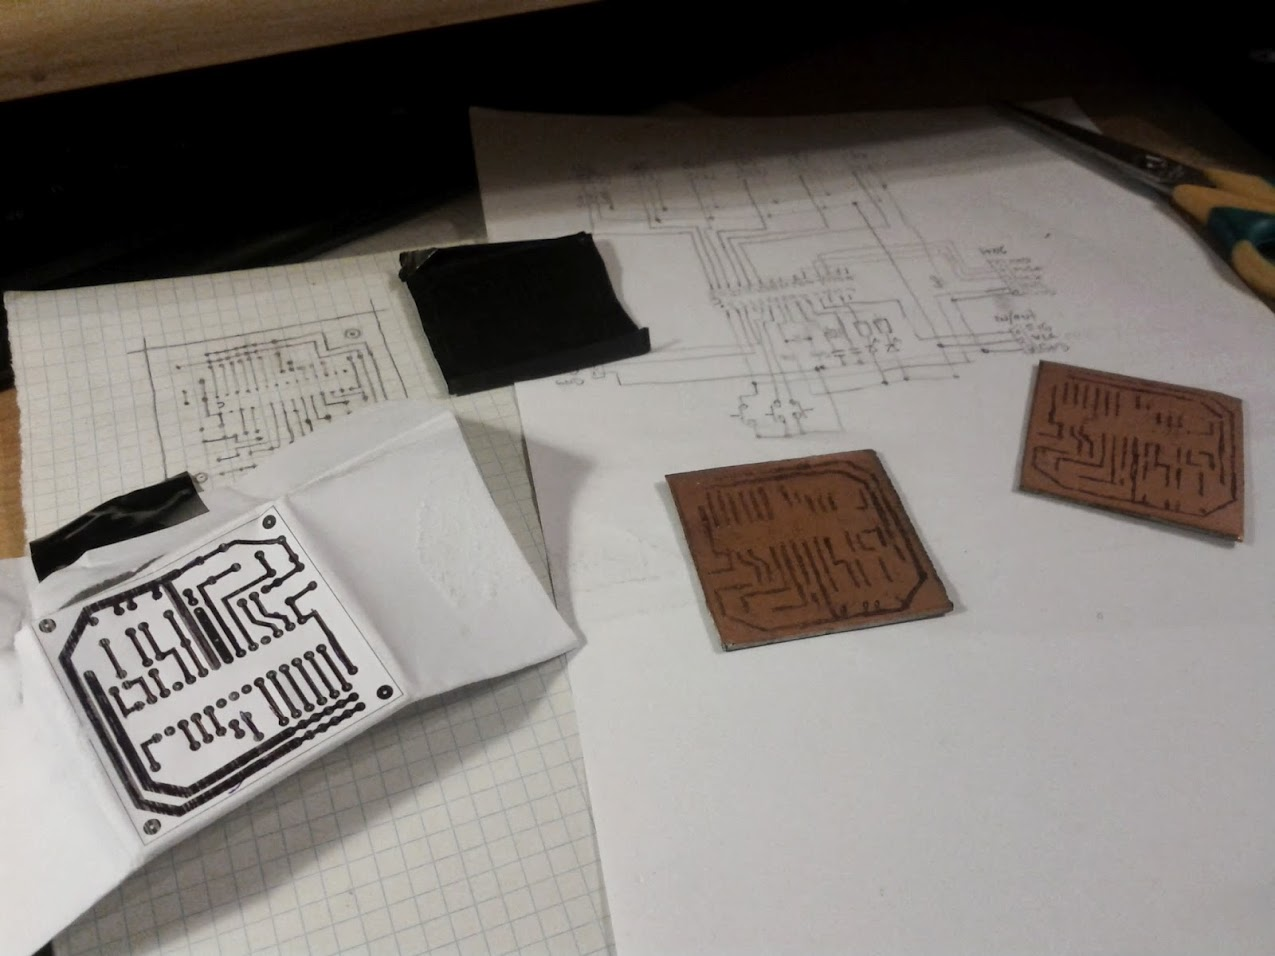
\includegraphics[width=0.85\textwidth]{./fig/pcb1.jpg}
  \end{figure}}

  \only<+>{\begin{figure}
      \caption{$\approx$ 2014, Model Predictive Control on embedded hardware}
      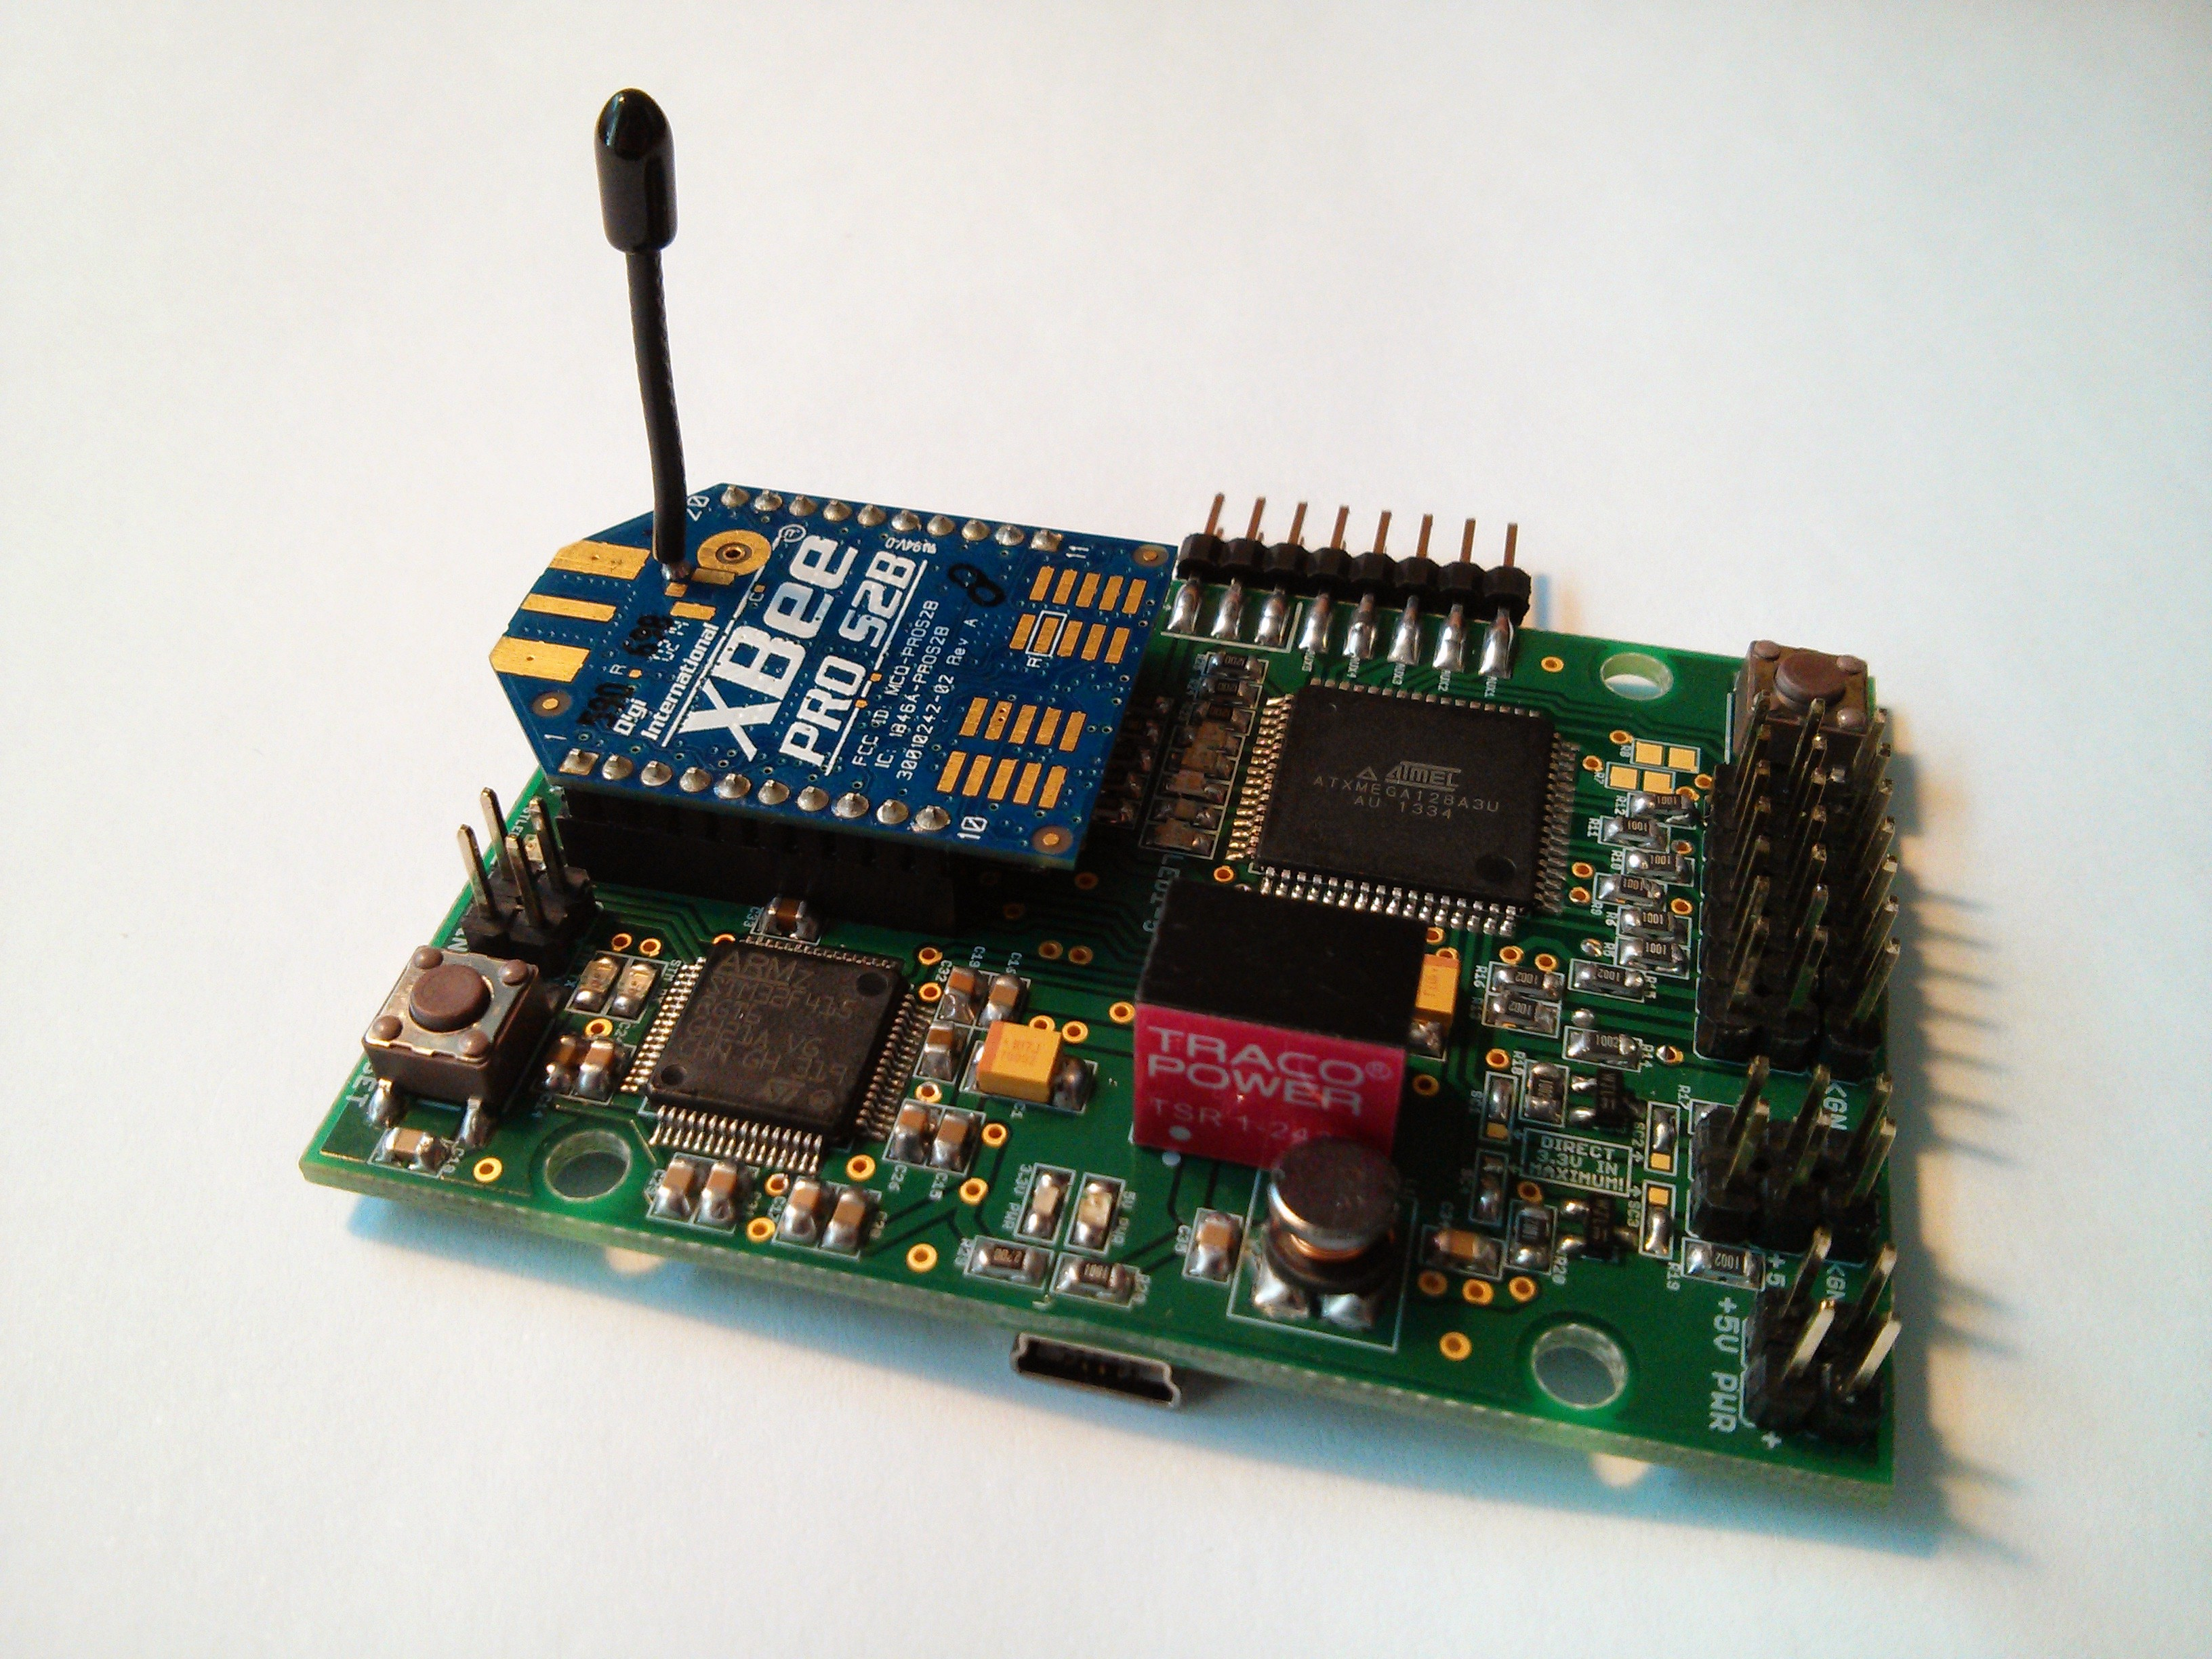
\includegraphics[width=0.85\textwidth]{./fig/pcb2.jpg}
  \end{figure}}

  \only<+>{\begin{figure}
      \caption{$\approx$ 2014, Model Predictive Control on embedded hardware}
      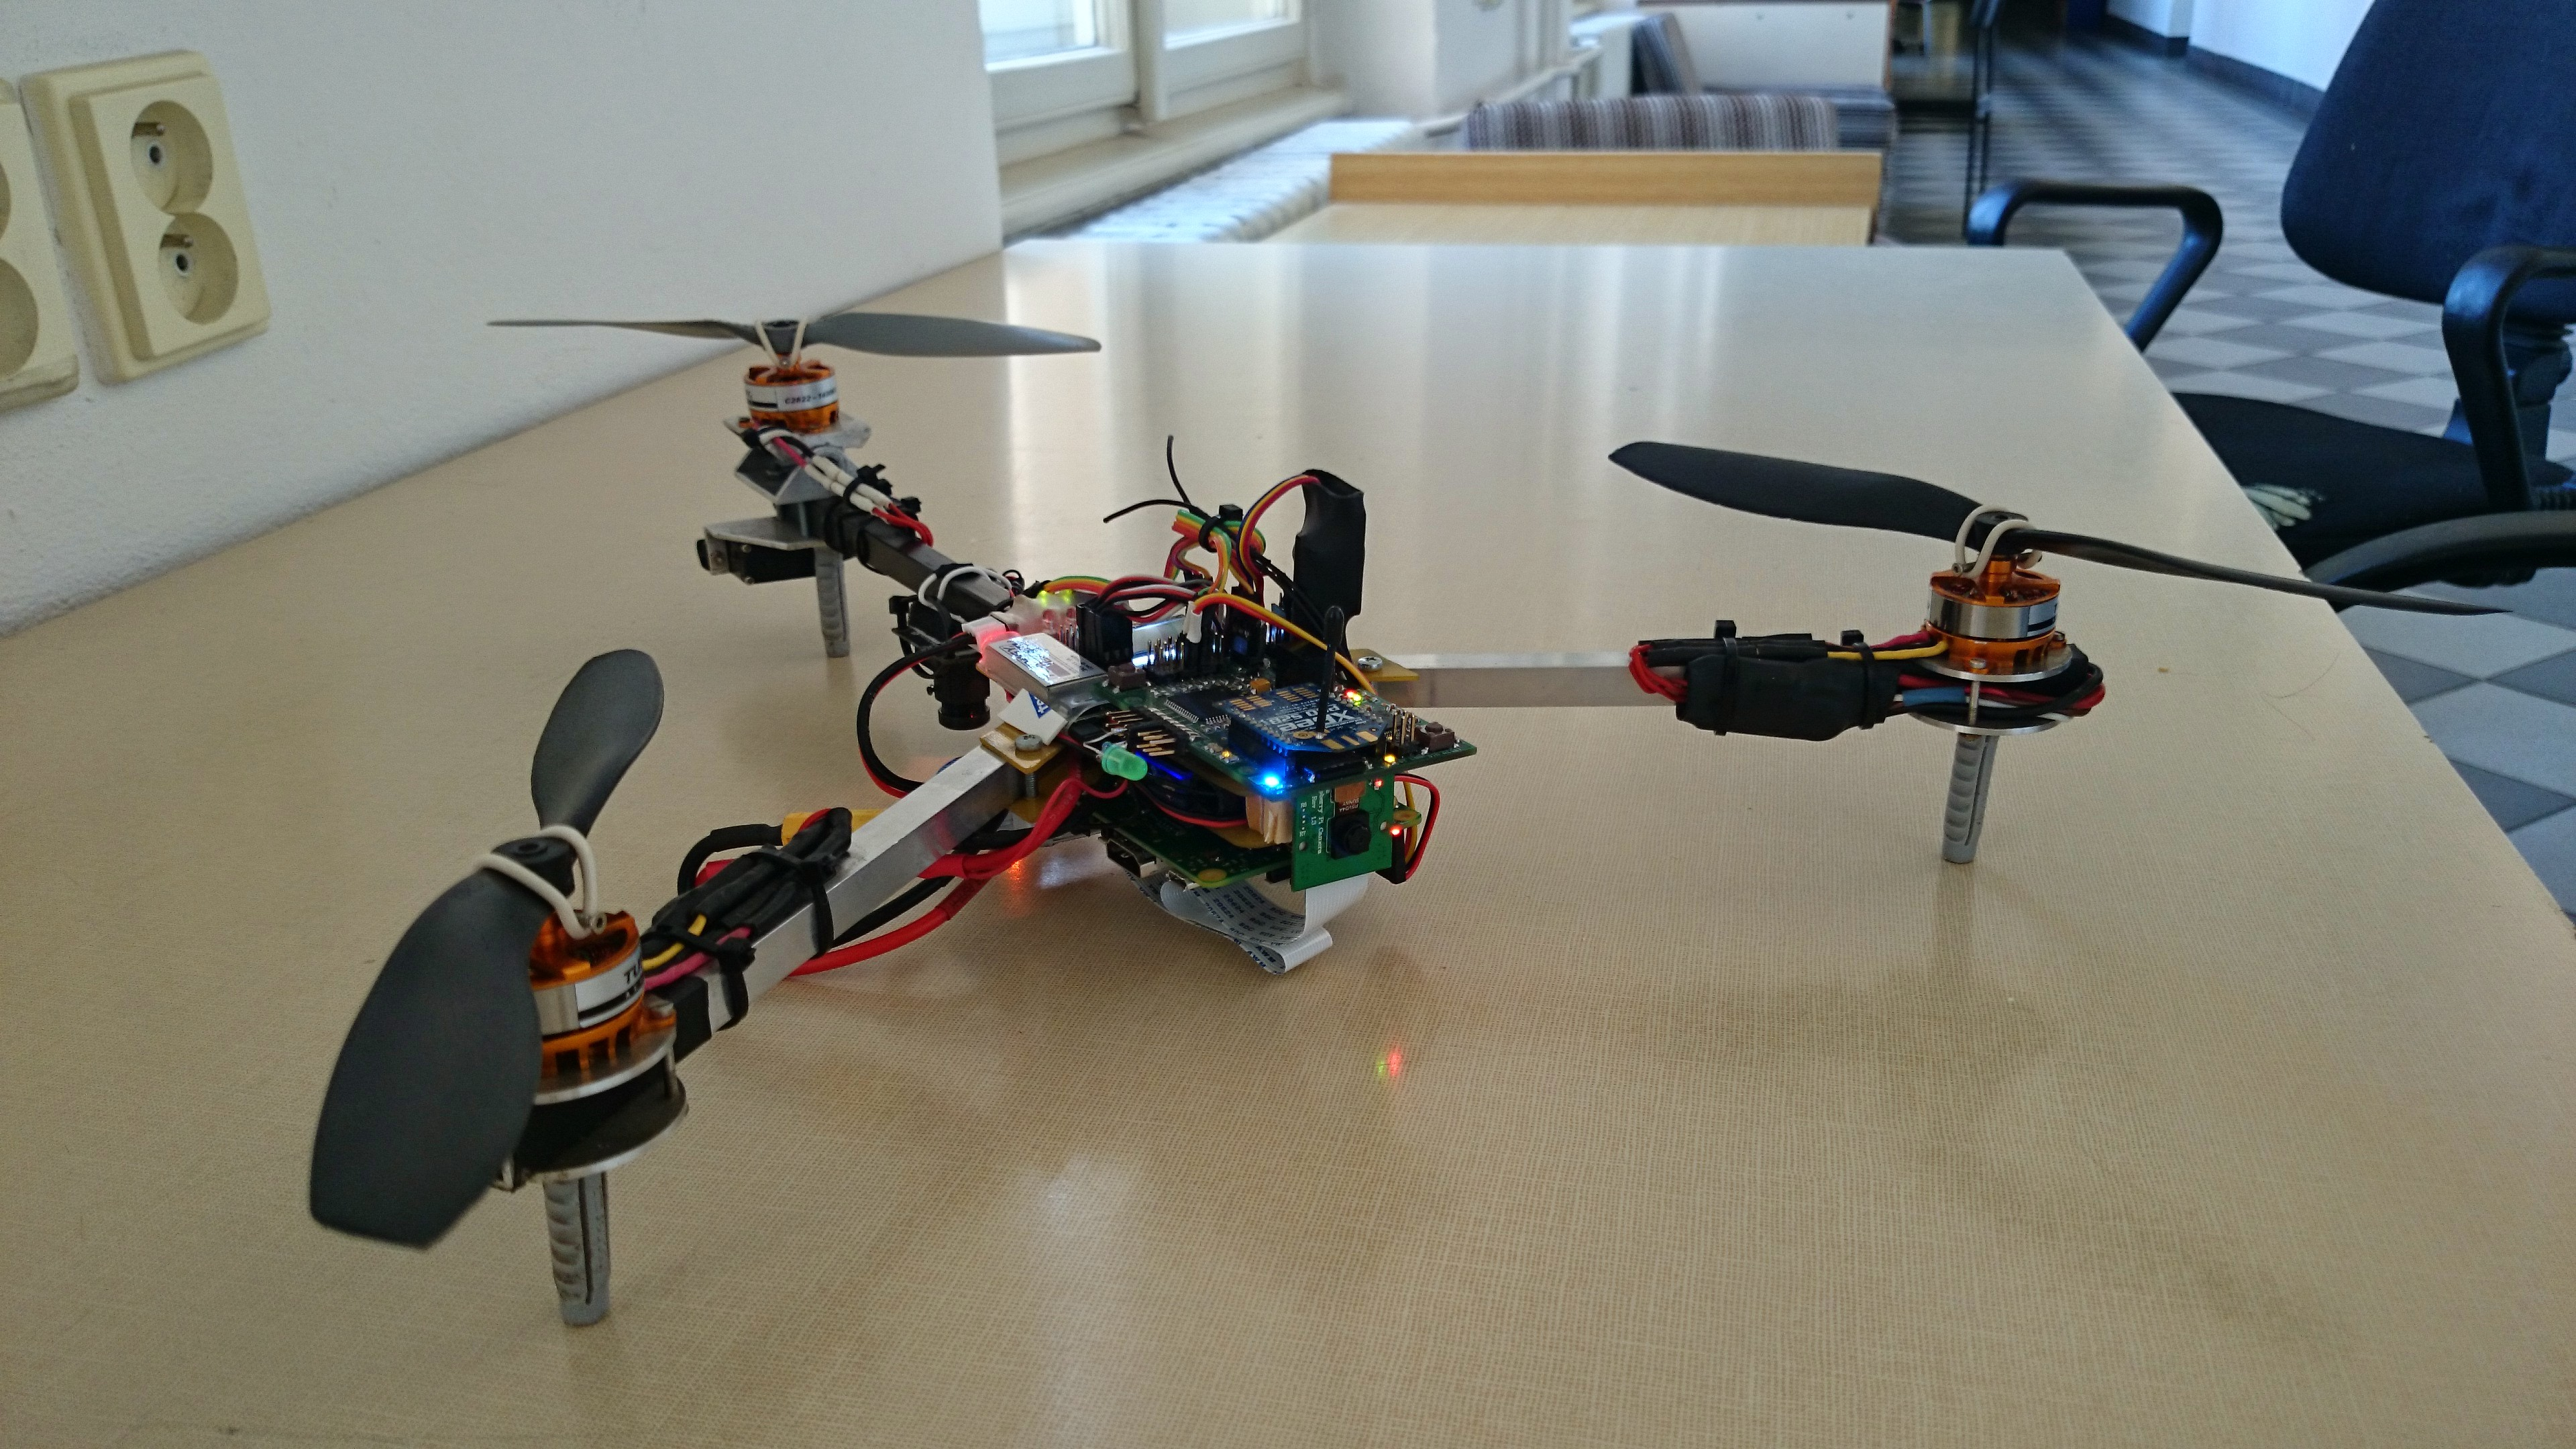
\includegraphics[width=0.85\textwidth]{./fig/tricopter.jpg}
  \end{figure}}

  \only<+>{\begin{block}{Embedded Model Predictive Control}
      \begin{center}
        \movie[externalviewer]{
          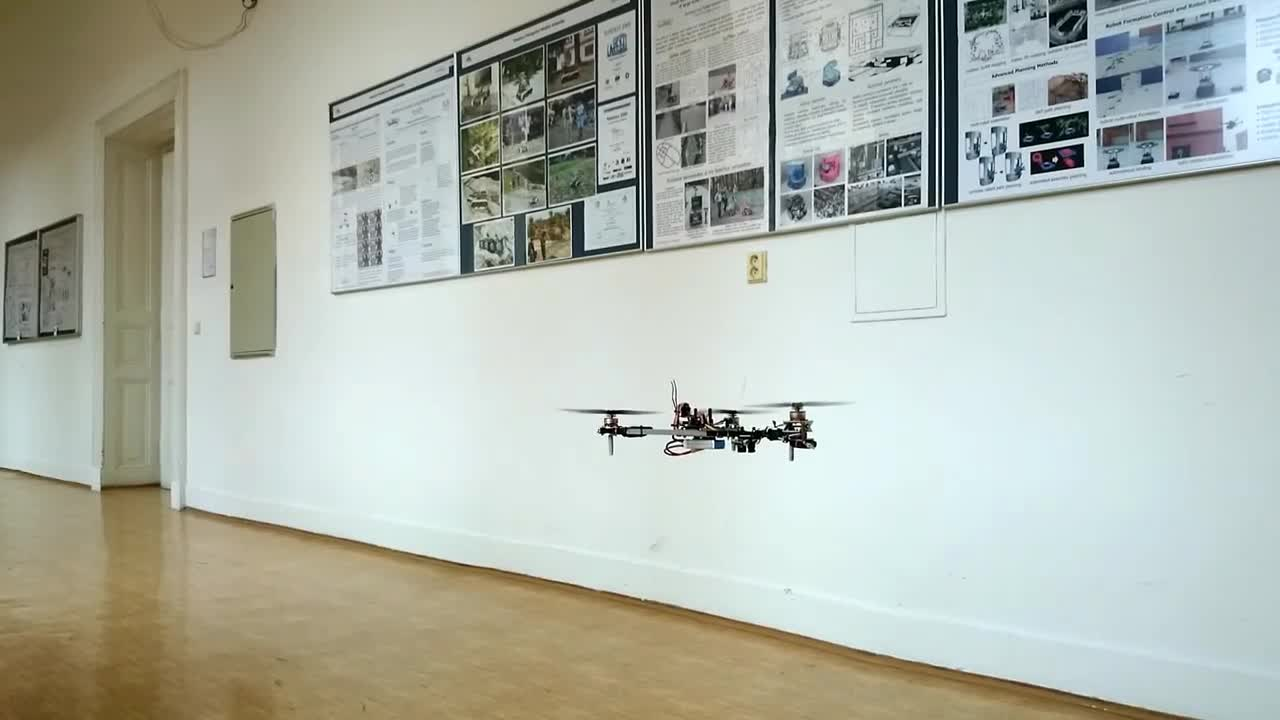
\includegraphics[width=0.9\textwidth]{./fig/embedded_mpc_thumbnail.jpg}
        }{../videos/embedded_mpc.mp4}\\
        Video: \url{https://youtu.be/AXI_rkQRBaE}
      \end{center}
  \end{block}}

\end{frame}

\begin{frame}
  \frametitle{A little bit of history}

  \begin{itemize}
    \onslide<1->{\item Custom and purpose-built hardware}
    \onslide<2->{\item Embedded software}
    \onslide<3->{\item Results: \\ Embedded MPC \cite{mmar_mpc}\\ Multi-robot publications: \cite{mmar_spurny}, \cite{auro}}
    \onslide<4->{\item ...}
    \onslide<5->{\item Not Scalable! Bottlenecks everywhere:}
    \onslide<6->{\item Embedded programming \emph{sucks}, simulations are difficult, system is hard to maintain, connecting sensors and peripheries is limited...}
    \onslide<7->{\item ... 2015}
\end{itemize}

\end{frame}

%%}

%%{ Nowadays
\begin{frame}
  \frametitle{Nowadays}

  \begin{figure}
    \caption{A typical pipeline structure revolves around a Linux computer.}
    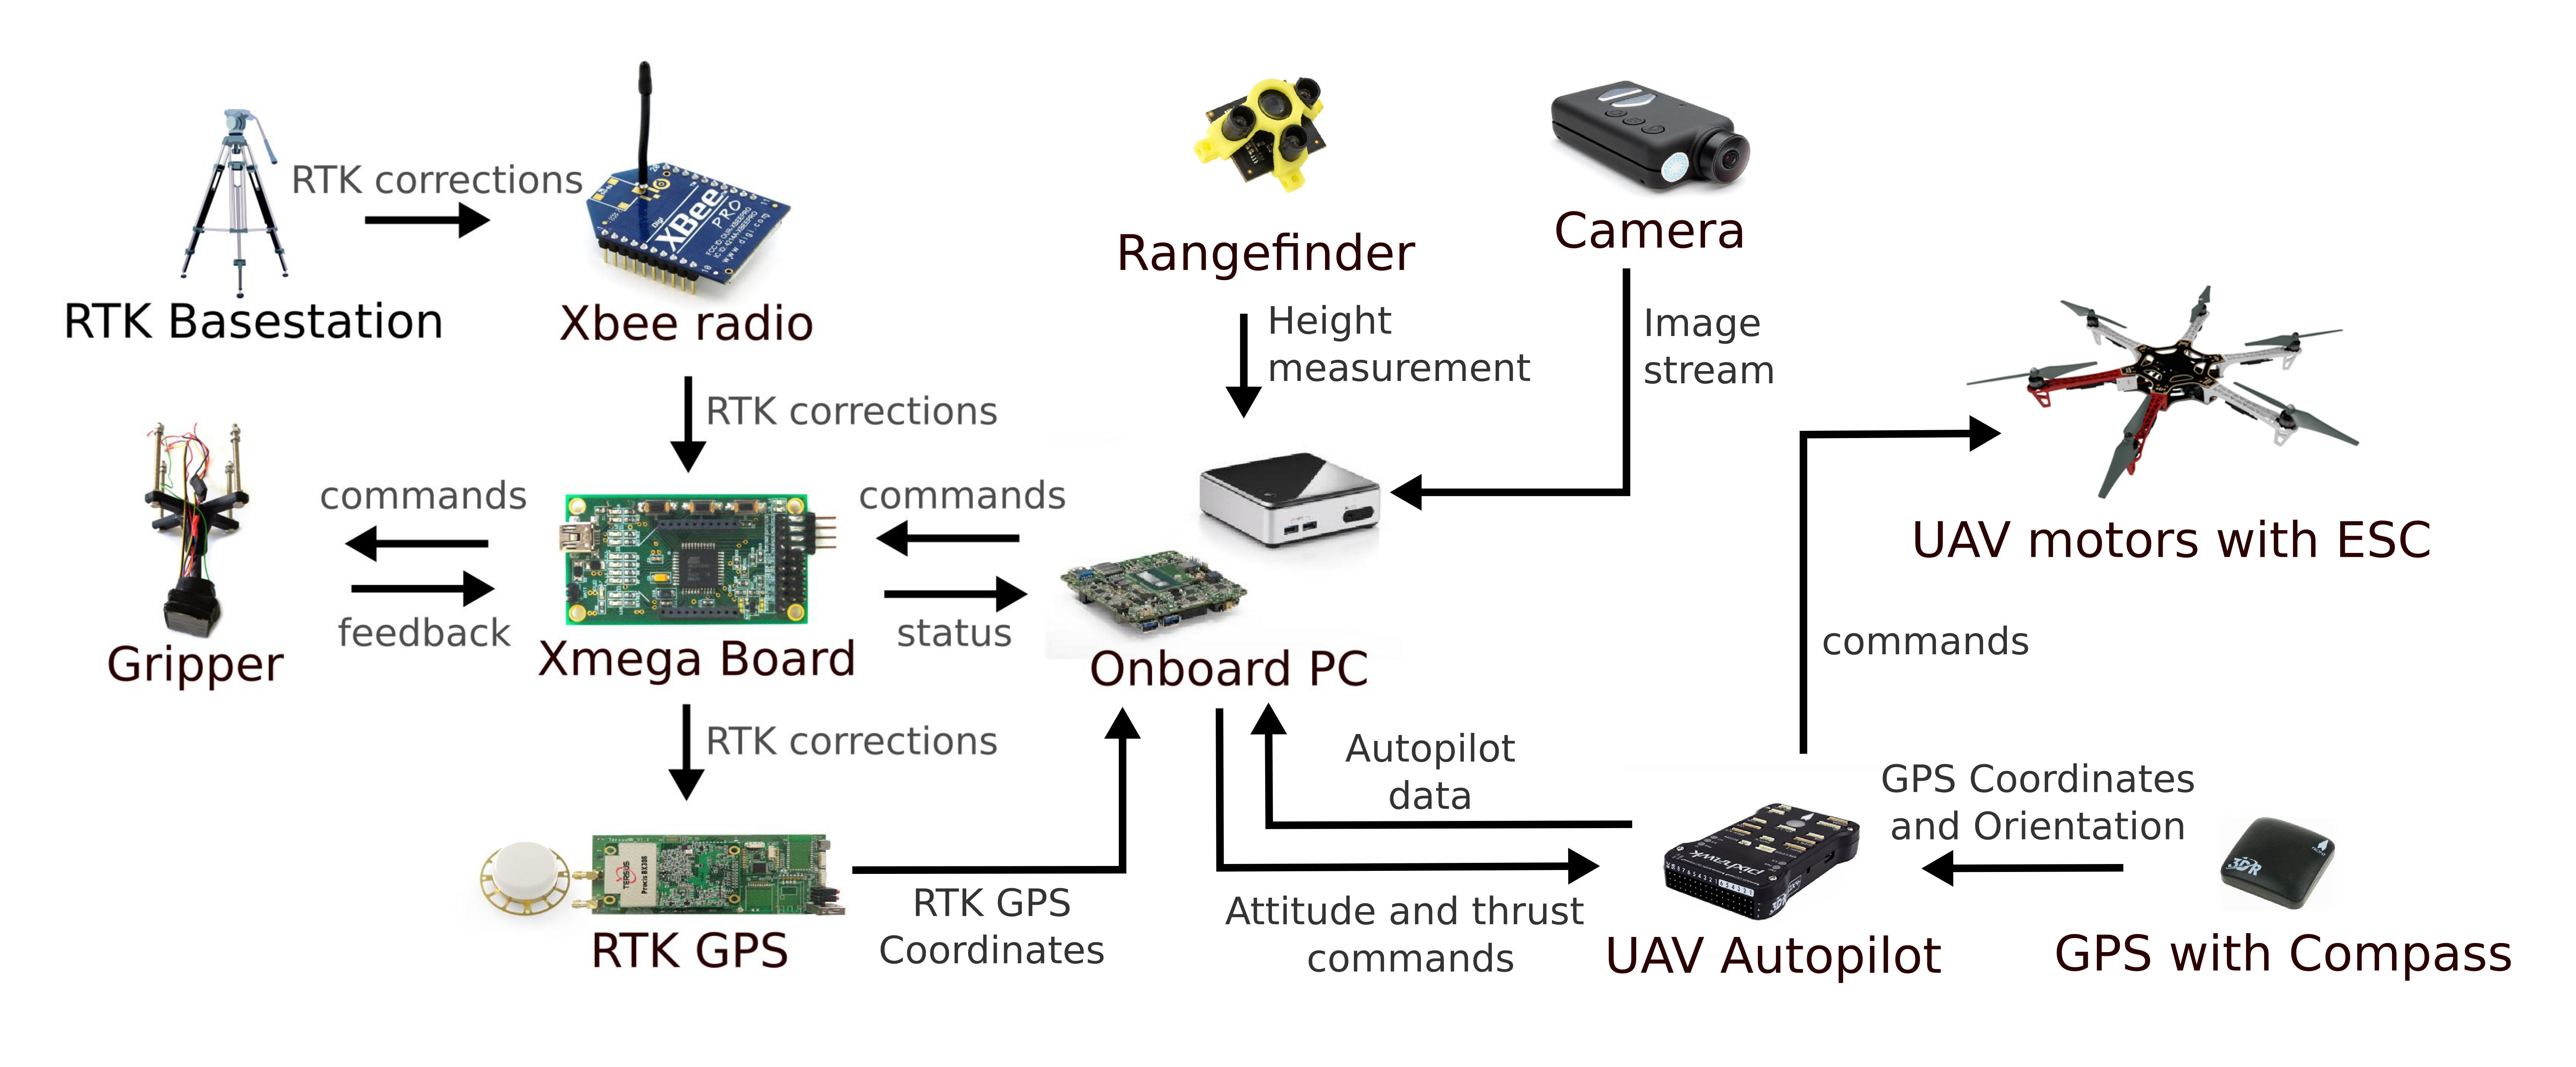
\includegraphics[width=1.0\textwidth]{./fig/components.png}
  \end{figure}

\end{frame}
%%}

%% --------------------------------------------------------------
%% |                    UAV control pipeline                    |
%% --------------------------------------------------------------

\section{UAV Control pipeline}
\subsection{control theory point of view}

%%{ UAV control pipepline
\begin{frame}
  \frametitle{Control -- theory POW}

  \centering
  \begin{figure}
    \begin{adjustbox}{max totalsize={1.0\textwidth}{.85\textheight}, center}
      \pgfdeclarelayer{foreground}
\pgfsetlayers{background,main,foreground}

\tikzset{radiation/.style={{decorate,decoration={expanding waves,angle=90,segment length=4pt}}}}

\begin{tikzpicture}[->,>=stealth', node distance=3.0cm,scale=1.0, every node/.style={scale=1.0}]

  %%{ nodes

  \node[state, shift = {(0.0, 0.0)}] (navigation) {
      \begin{tabular}{c}
        \footnotesize Mission \&\\
        \footnotesize navigation
      \end{tabular}
    };

  % \node[state, left of = navigation, shift = {(0.5, 0.0)}] (nimbro) {
  %     \begin{tabular}{c}
  %       \footnotesize Nimbro \\
  %       \footnotesize Network
  %     \end{tabular}
  %   };

  \node[state, right of = navigation, shift = {(0.7, 0)}] (tracker) {
      \begin{tabular}{c}
        \footnotesize Reference \\
        \footnotesize tracker
      \end{tabular}
    };

  \node[state, right of = tracker, shift = {(0.1, 0)}] (controller) {
      \begin{tabular}{c}
        \footnotesize Reference \\
        \footnotesize controller
      \end{tabular}
    };

  \node[state, right of = controller, shift = {(0.8, -0)}] (attitude) {
      \begin{tabular}{c}
        \footnotesize Attitude rate\\
        \footnotesize controller
      \end{tabular}
    };

  \node[state, right of = attitude, shift = {(0.7, -0)}] (actuators) {
      \begin{tabular}{c}
        \footnotesize UAV \\
        \footnotesize actuators
      \end{tabular}
    };

  \node[state, right of = actuators, shift = {(-1.0, -0)}] (sensors) {
      \begin{tabular}{c}
        \footnotesize Onboard \\
        \footnotesize sensors
      \end{tabular}
    };

  \node[state, below of = attitude, shift = {(0, 1.0)}] (estimator) {
      \begin{tabular}{c}
        \footnotesize State \\
        \footnotesize estimator
      \end{tabular}
    };

  %%}

  %%{ paths

  \path[->] ($(navigation.east) + (0.0, 0)$) edge [] node[above, midway, shift = {(0.0, 0.05)}] {
      \begin{tabular}{c}
        \footnotesize desired reference\\
        \footnotesize $\mathbf{r}_d, \eta_d$\\
        \footnotesize \textit{on demand}
    \end{tabular}} ($(tracker.west) + (0.0, 0.00)$);

  % \path[->] ($(nimbro.east) + (0.0, 0)$) edge [] node[above, midway, shift = {(0.0, 0.05)}] {
  %     \begin{tabular}{c}
  %   \end{tabular}} ($(navigation.west) + (0.0, 0.00)$);

  \path[->] ($(tracker.east) + (0.0, 0)$) edge [] node[above, midway, shift = {(0.0, 0.05)}] {
      \begin{tabular}{c}
        \footnotesize full-state reference\\
        \footnotesize $\bm{\chi}_d$\\
        \footnotesize \SI{100}{\hertz}
    \end{tabular}} ($(controller.west) + (0.0, 0.00)$);

  \path[->] ($(tracker.south |- estimator.west) + (0.0, 0.0)$) edge [dotted] node[left, midway, shift = {(0.2, 0.00)}] {
      \begin{tabular}{r}
        \scriptsize initialization\\[-0.5em]
        \scriptsize only
    \end{tabular}} ($(tracker.south) + (0.0, 0.00)$);

  \path[->] ($(controller.east) + (0.0, 0)$) edge [] node[above, midway, shift = {(-0.2, 0.05)}] {
      \begin{tabular}{c}
        \footnotesize $\bm{\omega}_d$\\
        \footnotesize $T_d$ \\
        \footnotesize \SI{100}{\hertz}
    \end{tabular}} ($(attitude.west) + (0.0, 0.00)$);

  \draw[-] ($(controller.south)+(0.25,0)$) -- ($(controller.south |- estimator.west) + (0.25, 0.25)$) edge [->] node[above, near start, shift = {(-0.2, 0.05)}] {
      \begin{tabular}{c}
        \footnotesize $\mathbf{a}_d$
    \end{tabular}} ($(estimator.west) + (0, 0.25)$);

  \path[->] ($(attitude.east) + (0.0, 0)$) edge [] node[above, midway, shift = {(0.1, 0.05)}] {
      \begin{tabular}{c}
        \footnotesize $\bm{\tau}_d$ \\
        \footnotesize $\approx$\SI{1}{\kilo\hertz}
    \end{tabular}} ($(actuators.west) + (0.0, 0.00)$);

  \path[-] ($(estimator.west)+(0, 0)$) edge [] node[above, near start, shift = {(-1.0, 0.0)}] {
      \begin{tabular}{c}
        \footnotesize $\mathbf{x}$, $\mathbf{R}$, $\bm{\omega}$\\
        \footnotesize \SI{100}{\hertz}
    \end{tabular}} ($(navigation.south |- estimator.west)$) -- ($(navigation.south |- estimator.west)$) edge [->,] ($(navigation.south)+(0, 0)$);

  % \path[-] ($(estimator.west)+(0, 0)$) edge [] node[above, near start, shift = {(-1.0, 0.0)}] {
  %     \begin{tabular}{c}
  %   \end{tabular}} ($(nimbro.south |- estimator.west)$) -- ($(nimbro.south |- estimator.west)$) edge [->,] ($(nimbro.south)+(0, 0)$);

  \path[->] ($(controller.south |- estimator.west)+(0, 0)$) edge [] ($(controller.south)$);

  \path[->] ($(attitude.south) + (0.0, -0.1)$) edge [] node[right, midway, shift = {(0.0, 0.00)}] {
      \begin{tabular}{c}
        \footnotesize $\mathbf{R}$, $\bm{\omega}$
    \end{tabular}} ($(estimator.north) + (0.0, 0.00)$);

  \path[-] ($(sensors.south)+(0, 0)$) edge [] ($(sensors.south |- estimator.east)$) -- ($(sensors.south |- estimator.east)$) edge [->,] node[above, near start, shift = {(-0.35, -0.1)}] {
      \begin{tabular}{c}
        \footnotesize onboard sensor data
    \end{tabular}}($(estimator.east)$);

  %%}

    % \draw[-, radiation, decoration={angle=45}] ($(nimbro.west) + (0.0, -0.0)$) -- +(0:-0.5);

  %%{ backgrounds

  \begin{pgfonlayer}{background}
    \path (attitude.west |- attitude.north)+(-0.45,0.8) node (a) {};
    \path (sensors.south -| sensors.east)+(+0.25,-0.20) node (b) {};
    \path[fill=gray!3,rounded corners, draw=black!70, densely dotted]
      (a) rectangle (b);
  \end{pgfonlayer}
  \node [rectangle, above of=actuators, shift={(-0.6,0.55)}, node distance=1.7em] (autopilot) {\footnotesize UAV plant};

  \begin{pgfonlayer}{background}
    \path (attitude.west |- attitude.north)+(-0.25,0.47) node (a) {};
    \path (attitude.south -| attitude.east)+(+0.25,-0.10) node (b) {};
    \path[fill=gray!3,rounded corners, draw=black!70, densely dotted]
      (a) rectangle (b);
  \end{pgfonlayer}
  \node [rectangle, above of=attitude, shift={(0,0.2)}, node distance=1.7em] (autopilot) {\footnotesize Embedded autopilot};

  %%}

\end{tikzpicture}

    \end{adjustbox}
  \end{figure}

  \begin{block}{\cite{iros}}
    Model Predictive Trajectory Tracking and Collision Avoidance for Reliable Outdoor Deployment of Unmanned Aerial Vehicles, IROS 2018.
  \end{block}

\end{frame}
%%}

\subsection{implementation point of view}

%%{ Control pipeline implementation
\begin{frame}
  \frametitle{Control -- implementation POW}

  \centering
  \begin{figure}
    \begin{adjustbox}{max totalsize={1.0\textwidth}{.85\textheight}, center}
      \pgfdeclarelayer{foreground}
\pgfsetlayers{background,main,foreground}

\tikzset{radiation/.style={{decorate,decoration={expanding waves,angle=90,segment length=0.1em}}}}

\begin{tikzpicture}[->,>=stealth', node distance=7.0em]

  \node[state_blue, shift = {(0.0em, 0.0em)}] (uav_manager) {
      \begin{tabular}{c}
        \small UAV manager
      \end{tabular}
    };

  \node[state_blue, below of = uav_manager, shift = {(0.0em, -0.0em)}] (control_manager) {
      \begin{tabular}{c}
        \small Control manager
      \end{tabular}
    };

  \node[state_red, right of = control_manager, shift = {(5.0em, 0.0em)}] (landoff_tracker) {
      \begin{tabular}{c}
        \small Landoff Tracker
      \end{tabular}
    };

  \node[state_red, below of = landoff_tracker, shift = {(0.0em, 4.5em)}] (mpc_tracker) {
      \begin{tabular}{c}
        \small MPC tracker
      \end{tabular}
    };

  \node[state_red, below of = mpc_tracker, shift = {(0.0em, 4.5em)}] (joy_tracker) {
      \begin{tabular}{c}
        \small Joy Tracker
      \end{tabular}
    };

  \node[state_red, below of = joy_tracker, shift = {(0.0em, 4.5em)}] (matlab_tracker) {
      \begin{tabular}{c}
        \small Matlab Tracker
      \end{tabular}
    };

  \node[state_red, below of = matlab_tracker, shift = {(0.0em, 4.5em)}] (csv_tracker) {
      \begin{tabular}{c}
        \small CSV tracker
      \end{tabular}
    };

  \node[state_green, left of = control_manager, shift = {(-5.0em, 0.0em)}] (so3_controller) {
      \begin{tabular}{c}
        \small SO(3) controller
      \end{tabular}
    };

  \node[state_green, below of = so3_controller, shift = {(0.0em, 4.5em)}] (mpc_controller) {
      \begin{tabular}{c}
        \small MPC controller
      \end{tabular}
    };

  \node[state_blue, above of = so3_controller, shift = {(0.0em, -2.0em)}] (gain_manager) {
      \begin{tabular}{c}
        \small Gain manager
      \end{tabular}
    };

  \node[state_green, below of = mpc_controller, shift = {(0.0em, 4.5em)}] (failsafe_controller) {
      \begin{tabular}{c}
        \small Failsafe controller
      \end{tabular}
    };

  \node[state_green, below of = failsafe_controller, shift = {(0.0em, 4.5em)}] (nsf_controller) {
      \begin{tabular}{c}
        \small NSF conroller
      \end{tabular}
    };

  \node[state_green, below of = nsf_controller, shift = {(0.0em, 4.5em)}] (attitude_controller) {
      \begin{tabular}{c}
        \small Attitude controller
      \end{tabular}
    };

  \node[state_blue, above of = landoff_tracker, shift = {(0.0em, -2.0em)}] (constraint_manager) {
      \begin{tabular}{c}
        \small Constraint manager
      \end{tabular}
    };

  \node[state, below of = control_manager, shift = {(4.0em, 0.0em)}] (mavros2) {
      \begin{tabular}{c}
        \small Mavros
      \end{tabular}
    };

  \node[state, below of = mavros2, shift = {(0.0em, 4.5em)}] (pixhawk2) {
      \begin{tabular}{c}
        \small Pixhawk
      \end{tabular}
    };

  \node[state_white, below of = control_manager, shift = {(0.0em, -6.0em)}] (odometry) {
      \begin{tabular}{c}
        \small Odometry
      \end{tabular}
    };

  \node[state, left of = odometry, shift = {(-5.0em, -2.0em)}] (bumper) {
      \begin{tabular}{c}
        \small Obstacle bumper
      \end{tabular}
    };

  \node[state, below of = odometry, shift = {(0.0em, 0.0em)}] (mavros_interface) {
      \begin{tabular}{c}
        \small Mavros interface
      \end{tabular}
    };

  \node[state, below of = mavros_interface, shift = {(0.0em, 4.5em)}] (mavros) {
      \begin{tabular}{c}
        \small Mavros
      \end{tabular}
    };

  \node[state_gray, below of = mavros, shift = {(0.0em, 4.5em)}] (pixhawk) {
      \begin{tabular}{c}
        \small Pixhawk
      \end{tabular}
    };

  \node[state, right of = mavros_interface, shift = {(0.0em, 0.0em)}] (optic_flow) {
      \begin{tabular}{c}
        \small Optic flow
      \end{tabular}
    };

  \node[state, below of = optic_flow, shift = {(0.0em, 4.5em)}] (auto_exposure) {
      \begin{tabular}{c}
        \small Auto exposure
      \end{tabular}
    };

  \node[state_gray, below of = auto_exposure, shift = {(0.0em, 4.5em)}] (bluefox) {
      \begin{tabular}{c}
        \small Bluefox
      \end{tabular}
    };

  \node[state_gray, left of = mavros_interface, shift = {(0.0em, 0.0em)}] (garmin) {
      \begin{tabular}{c}
        \small Garmin
      \end{tabular}
    };

  \node[state_gray, left of = garmin, shift = {(0.0em, 0.0em)}] (rplidar) {
      \begin{tabular}{c}
        \small Rplidar
      \end{tabular}
    };

  \node[state_gray, right of = optic_flow, shift = {(1.0em, 0.0em)}] (realsense) {
      \begin{tabular}{c}
        \small Realsense
      \end{tabular}
    };

  \node[state, above of = realsense, shift = {(0.0em, -3.5em)}] (orb_slab) {
      \begin{tabular}{c}
        \small ORB slam
      \end{tabular}
    };

    %% | ---------- connections from sensors to odometry ---------- |
    \path[-] ($(rplidar.north)$) edge [->] ($(odometry.south) + (-1em, 0)$);
    \path[-] ($(garmin.north)$) edge [->] ($(odometry.south) + (-0.5em, 0)$);
    \path[-] ($(mavros_interface.north)$) edge [->] ($(odometry.south) + (0, 0)$);
    \path[-] ($(optic_flow.north)$) edge [->] ($(odometry.south) + (0.5em, 0)$);
    \path[-] ($(orb_slab.west)$) edge [->] ($(odometry.south) + (1em, 0)$);

    \path[-] ($(mavros.north)$) edge [->] ($(mavros_interface.south)$);
    \path[-] ($(bluefox.north)$) edge [->] ($(auto_exposure.south)$);
    \path[-] ($(auto_exposure.north)$) edge [->] ($(optic_flow.south)$);
    \draw[->] ($(bluefox.east)$) -- +(2em, 0) |- ($(optic_flow.east)$);

    %% | ------------------ orb slam to realsense ----------------- |
    \path[-] ($(realsense.north)$) edge [->] ($(orb_slab.south)$);

    %% | ----- connections from controllers to control manager ---- |
    \path ($(so3_controller.east)$) edge [<->] ($(control_manager.west) + (0, 0.4em)$);
    \path ($(mpc_controller.east)$) edge [<->] ($(control_manager.west) + (0, 0.20em)$);
    \path ($(failsafe_controller.east)$) edge [<->] ($(control_manager.west) + (0, 0.0em)$);
    \path ($(nsf_controller.east)$) edge [<->] ($(control_manager.west) + (0, -0.20em)$);
    \path ($(attitude_controller.east)$) edge [<->] ($(control_manager.west) + (0, -0.40em)$);

    %% | ------ connections from trackers to control manager ------ |
    \path ($(landoff_tracker.west)$) edge [<->] ($(control_manager.east) + (0, 0.40em)$);
    \path ($(mpc_tracker.west)$) edge [<->] ($(control_manager.east) + (0, 0.20em)$);
    \path ($(joy_tracker.west)$) edge [<->] ($(control_manager.east) + (0, 0.00em)$);
    \path ($(matlab_tracker.west)$) edge [<->] ($(control_manager.east) + (0, -0.20em)$);
    \path ($(csv_tracker.west)$) edge [<->] ($(control_manager.east) + (0, -0.40em)$);

    %% | ------------------- gain manager to so3 ------------------ |
    \path[-] ($(gain_manager.south)$) edge [->] ($(so3_controller.north)$);

    %% | ---------- constraint manager to control manager --------- |
    \draw[<-] ($(constraint_manager.west)$) -- ($(control_manager.north |- constraint_manager.west) + (2em, 0)$) edge [->] ($(control_manager.north) + (2em, 0)$);
    \draw[<-] ($(gain_manager.east)$) -- ($(control_manager.north |- constraint_manager.east) + (-2em, 0)$) edge [->] ($(control_manager.north) + (-2em, 0)$);

    %% | ------------- control manager to uav manager ------------- |
    \path ($(uav_manager.south)$) edge [<->] ($(control_manager.north)$);

    %% | --------------- odometry to control manager -------------- |
    \path ($(odometry.north)$) edge [<->] ($(control_manager.south)$);

    %% | ------------------------- pixhawk ------------------------ |
    \path ($(pixhawk.north)$) edge [->] ($(mavros.south)$);

    %% | ------------------------ pixhawk 2 ----------------------- |
    \path ($(control_manager.south) + (2em, 0)$) edge [->] ($(mavros2.north)$);
    \path ($(pixhawk2.north)$) edge [<-] ($(mavros2.south)$);

    %% | --------------------- obstacle bumper -------------------- |
    \path ($(rplidar.north)$) edge [<->] ($(bumper.south)$);
    \path ($(bumper.east)$) edge [<->] ($(control_manager.south) + (-4em, 0)$);

\end{tikzpicture}

    \end{adjustbox}
  \end{figure}

\end{frame}
%%}

%% --------------------------------------------------------------
%% |                      Linux environment                     |
%% --------------------------------------------------------------

\section{Linux technologies}
\subsection{terminal, shell, TMUX, Vim, ROS}

%%{ Linux terminal & shell
\begin{frame}
  \frametitle{Linux terminal \& shell}

  \begin{figure}
    \caption{A Linux terminal}
    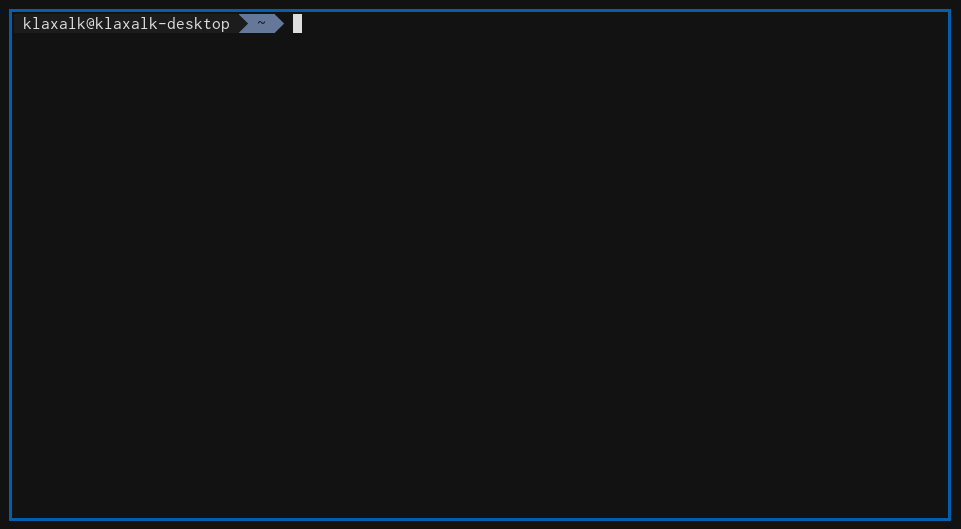
\includegraphics[width=1.0\textwidth]{./fig/terminal.png}
  \end{figure}

\end{frame}
%%}

%%{ Tmux & Terminal multiplexer
\begin{frame}

  \frametitle{Tmux -- Terminal multiplexer}

  \begin{figure}
    \caption{A Linux terminal with Tmux}
    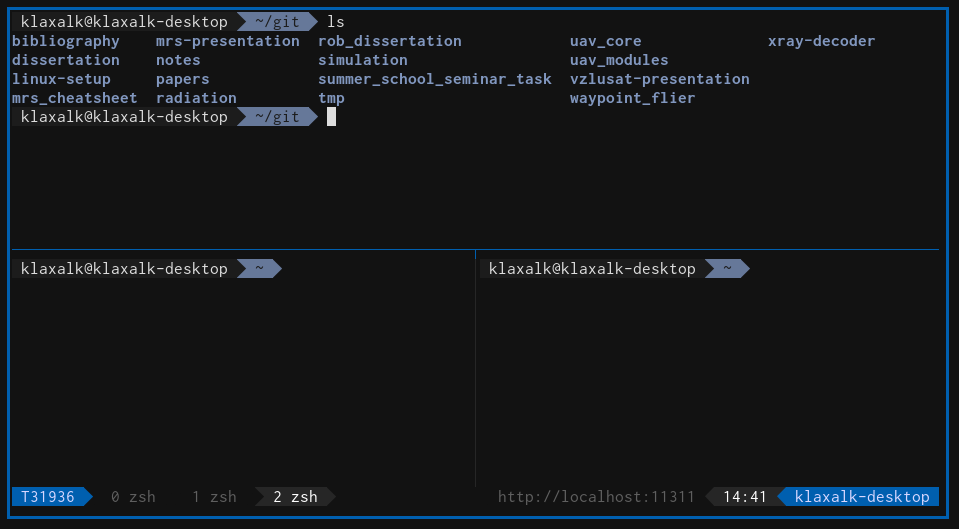
\includegraphics[width=1.0\textwidth]{./fig/tmux.png}
  \end{figure}

\end{frame}
%%}

%%{ Vim -- modal, modular, modern
\begin{frame}
  \frametitle{Vim -- modal, modular, modern}

  \begin{figure}
    \caption{Vim in Tmux in Terminal}
    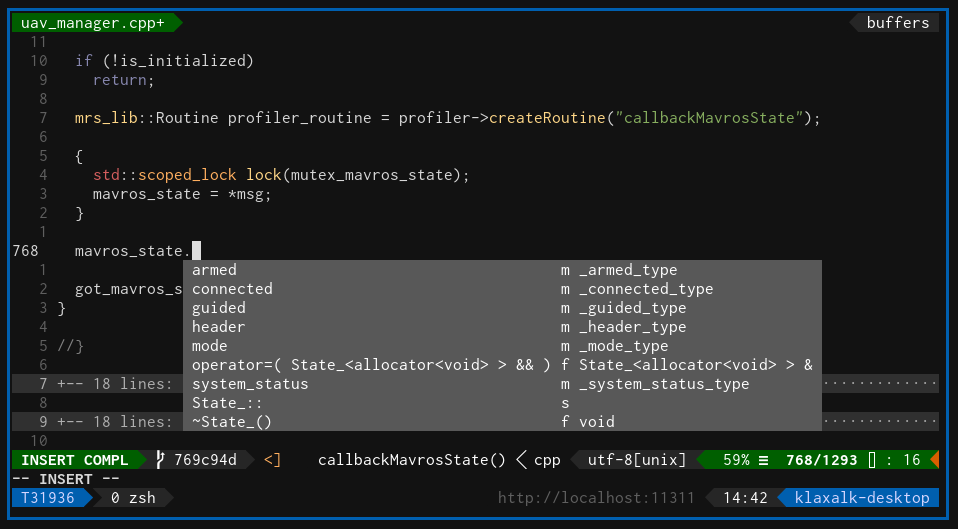
\includegraphics[width=1.0\textwidth]{./fig/vim.png}
  \end{figure}

\end{frame}
%%}

%%{ ROS -- Robot Operating System
\begin{frame}
  \frametitle{ROS -- Robot Operating System}

  \begin{itemize}
    \item Middleware allowing communication between programs
    \item Makes the transition from \emph{Matlab} to reality bearable
    \item Supported by sensor manufacturers (lots of ROS drivers)
    \item Integration through the terminal (important, works over ssh)
    \item Handles the difficult stuff nobody that wants to program: time management, logging, recording onboard data, common visualization, parameter loading, static and dynamic transformations, etc.
    \item integrates to most robotic simulators: Gazebo, Vrap
  \end{itemize}

\end{frame}
%%}

%% | ---------------------- The simulator --------------------- |

\section{MRS simulation stack}

\subsection{Gazebo/ROS, spawn}

%%{ Gazebo/ROS simulator
\begin{frame}
  \frametitle{Gazebo/ROS simulator}



\end{frame}
%%}

%%{ Spawning drones to the simulator
\begin{frame}
  \frametitle{Spawning drones to the simulator}



\end{frame}
%%}

%% | ------------------ Seminars assignments ------------------ |

\section{Summer School seminar}
\subsection{the MTSPN problem}
\subsection{running the planner, w/ and w/o ROS}

\subsection{running the simulation}

%% --------------------------------------------------------------
%% |                          resources                         |
%% --------------------------------------------------------------

%%{ MRS wiki
\begin{frame}
  \frametitle{MRS wiki}

  \begin{figure}
    \caption*{\url{https://mrs.felk.cvut.cz/gitlab/uav/uav_core/wikis/home}}
    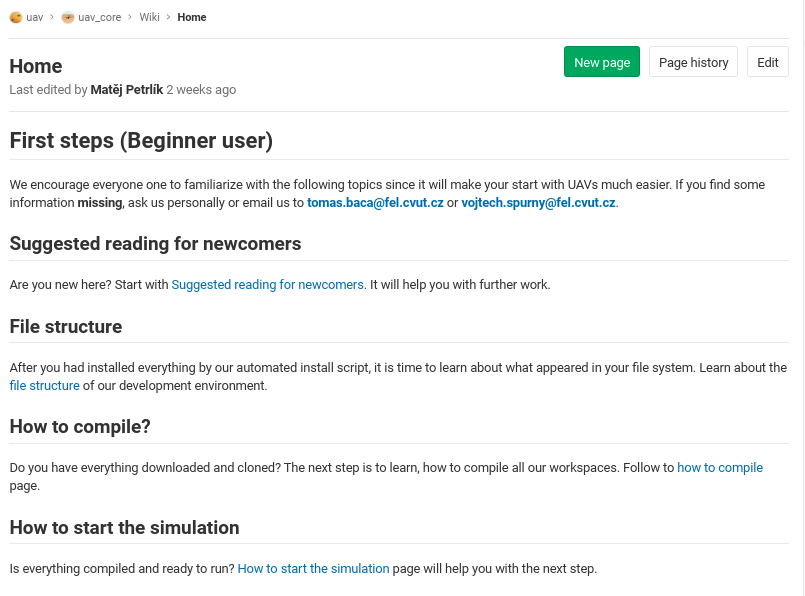
\includegraphics[width=0.9\textwidth]{./fig/wiki.png}
  \end{figure}

\end{frame}
%%}

%%{ MRS Cheat Sheet
\begin{frame}
  \frametitle{MRS Cheat Sheet}

  \begin{figure}
    \caption*{\url{https://github.com/klaxalk/mrs-cheatsheet}}
    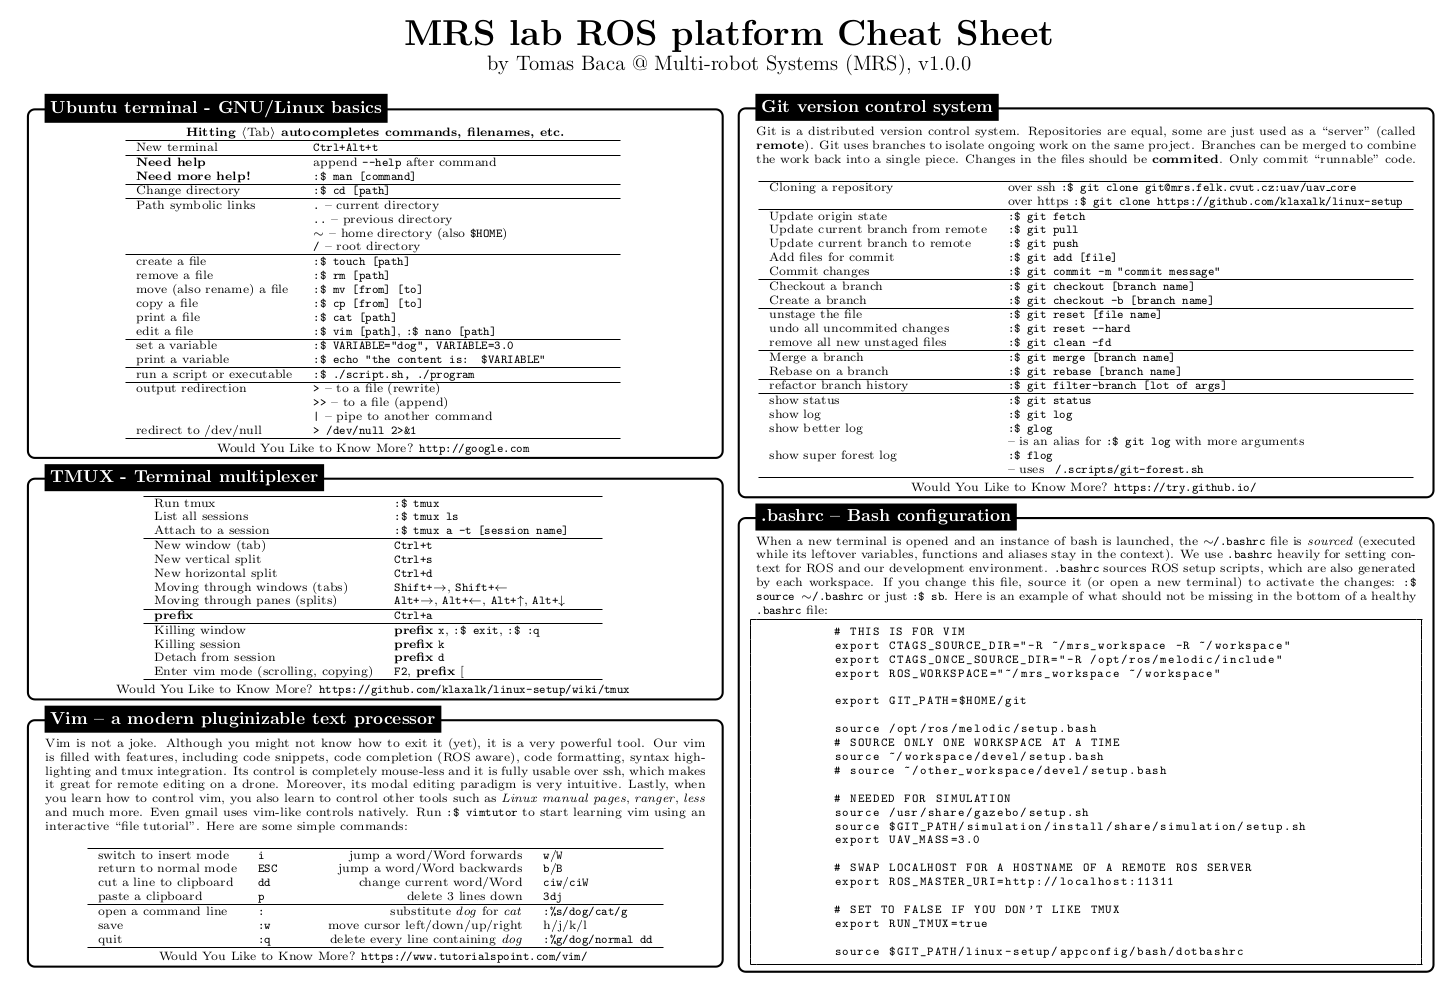
\includegraphics[width=0.9\textwidth]{./fig/mrs_cheatsheet.png}
  \end{figure}

\end{frame}
%%}

%%{ Links
\begin{frame}
  \frametitle{Links}

  \begin{itemize}
    \item Linux setup -- \\\url{https://github.com/klaxalk/linux-setup}
    \item MRS cheat sheet -- \\\url{https://github.com/klaxalk/mrs-cheatsheet}
    \item This presentation -- \\\url{https://github.com/klaxalk/mrs-presentation}
  \end{itemize}

\end{frame}
%%}

%%{ REFERENCES

\begin{frame}
  \frametitle{References}
  \tiny{
    \begin{thebibliography}{99}

      \bibitem[Baca et al., 2016]{mmar_mpc} Baca, T and Loianno, G and Saska, M
      \newblock Embedded Model Predictive Control of Unmanned Micro Aerial Vehicles
      \newblock 2016 IEEE International Conference on Methods and Models in Automation

      \bibitem[Spurny et al., 2016]{mmar_spurny} Spurny, V and Baca, T and Saska, M
      \newblock Complex manoeuvres of heterogeneous MAV-UGV formations using a model predictive control
      \newblock 2016 IEEE International Conference on Methods and Models in Automation

      \bibitem[Saska et al, 2016]{auro} Saska, M and Baca, T and Thomas, J and Chudoba, J and Preucil, L and Krajnik, T and Faigl, J and Loianno, G and Kumar, V
      \newblock System for deployment of groups of unmanned micro aerial vehicles in GPS-denied environments using onboard visual relative localization
      \newblock Autonomous Robots, 2016

      \bibitem[Baca et al., 2018]{iros} Baca, T and Hert, D and Loianno, G and Saska, M and Kumar, V
      \newblock Model Predictive Trajectory Tracking and Collision Avoidance for Reliable Outdoor Deployment of Unmanned Aerial Vehicles
      \newblock 2018 IEEE/RSJ International Conference on Intelligent Robots and Systems

  \end{thebibliography}
}
\end{frame}

%%}

  \end{document}
